%!TEX TS-program = xelatex

\documentclass {beamer}

%\input {inc0gnito.sty}

\useoutertheme{infolines}

\usepackage{xetexko}
\usepackage{mathtools}
\usepackage{amsmath}
\usepackage{fontspec}
\usepackage{hyperref}
\usepackage{graphicx}
\usepackage{listings}
\usepackage{makeidx}
\usepackage{indentfirst}
\usepackage{standalone}


%\setmainfont {NanumMyeongjo}
\setsansfont {Noto Sans CJK KR}
\setmainfont {Noto Sans CJK KR}
\setmonofont[Scale=0.8]{DejaVu Sans Mono}

\lstdefinestyle{diff}{
  belowcaptionskip=1\baselineskip,
  breaklines=true,
  frame=L,
  xleftmargin=\parindent,
  showstringspaces=false,
  % Diffstart
  morecomment=[f][\color{gray}]{@@},
  % Diffincl
  morecomment=[f][\color{Green}]{+},
  % Diffrem
  morecomment=[f][\color{Red}]{-},
  basicstyle=\footnotesize\ttfamily,
}

\lstdefinestyle{customtxt}{
  belowcaptionskip=1\baselineskip,
  breaklines=true,
  frame=L,
  xleftmargin=\parindent,
  showstringspaces=false,
  basicstyle=\footnotesize\ttfamily,
}

\lstdefinestyle{customc}{
  belowcaptionskip=1\baselineskip,
  breaklines=true,
  frame=L,
  xleftmargin=\parindent,
  language=C,
  showstringspaces=false,
  basicstyle=\footnotesize\ttfamily,
  keywordstyle=\bfseries\color{green!40!black},
  commentstyle=\itshape\color{purple!40!black},
  identifierstyle=\color{blue},
  stringstyle=\color{orange},
}


\hypersetup {
  colorlinks, linkcolor=blue
}

\title {K-공유기 씹고 뜯고 맛보고 즐기기}
\author {perillamint}


\AtBeginSection[]
{
  \begin{frame}
    \frametitle{Index}
    \tableofcontents[currentsection]
  \end{frame}
}

\begin {document}

\begin{frame}
  \titlepage
\end{frame}

%아 일하기 싫다 진짜 싫다 귀찮다 자고싶다

\section[Section]{K-공유기?}
\begin{frame}
  \frametitle{0x00. K-공유기?}
  \framesubtitle{*NIX 셸 스크립트 두 명 타요}

  \begin{itemize}
  \item 대부분의 가정마다 한 대쯤은 있는 물건
  \item<2-> 하지만, 대부분의 소비자는 공유기의 품질에 대해 신경쓰지 않음
  \item<3-> 기업은 원가를 절감하기 위해, 하드웨어와 소프트웨어에 대한 투자를 줄임
  \end{itemize}
\end{frame}

\begin{frame}
  \frametitle{0x00. K-공유기?}
  \framesubtitle{*NIX 셸 스크립트 두 명 타요}

  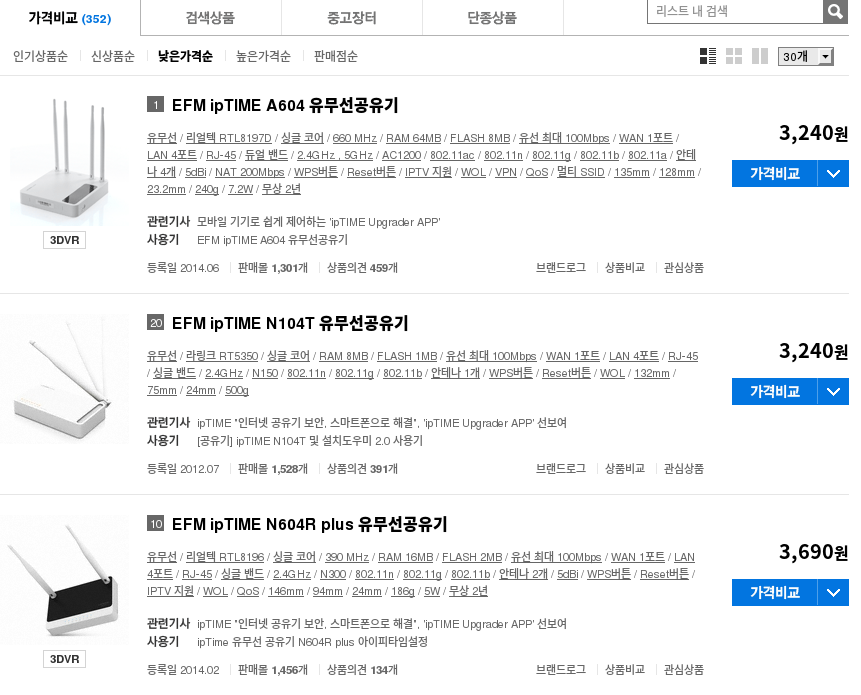
\includegraphics [width=90mm]{img/cheapwrt.png}
\end{frame}

\begin{frame}
  \frametitle{0x00. K-공유기?}
  \framesubtitle{*NIX 셸 스크립트 두 명 타요}

  \begin{itemize}
  \item 대부분의 가정마다 한 대쯤은 있는 물건
  \item 하지만, 대부분의 소비자는 공유기의 품질에 대해 신경쓰지 않음
  \item 기업은 원가를 절감하기 위해, 하드웨어와 소프트웨어에 대한 투자를 줄임
  \item 저렴한 개발자들은, 시큐어 코딩의 필요성을 잘 못 느낌.
  \item<2-> 털기 쉬울것 같다. 열어보자
  \end{itemize}
\end{frame}

\section[Section]{취약점 공략 포인트}
\begin{frame}
  \frametitle{0x01. 취약점 공략 포인트}
  \framesubtitle{공격 벡터가 될 수 있을 만한 것은?}

  \begin{itemize}
  \item 공유기, aka. 홈 라우터의 하는 일은?
  \item<2-> 라우팅
  \item<2-> Network Address Translation
  \item<2-> \textbf{웹 관리 인터페이스 서빙}
  \end{itemize}
\end{frame}

\begin{frame}
  \frametitle{0x01. 취약점 공략 포인트}
  \framesubtitle{Running everything as a root is a bad idea.}

  \begin{itemize}
  \item 공유기의 웹 관리 인터페이스는 공유기의 라우팅, NAT 등의 설정을 건드릴 수 있다.
  \item<2-> HTTP 데몬이 루트 권한으로 동작한다면, 쉽게 /proc /sys 의 파일들을 조작하고 iptables 명령을 실행할 수 있을 것이다.
  \item<2-> 아마도 제조사들은 이 방식으로 웹 관리 페이지를 구현했을 것이다.
  \item<3-> \textbf{HTTP 데몬을 공략하자}.
  \end{itemize}
\end{frame}

\section[Section]{데이터 추출}
\begin{frame}
  \frametitle{0x02. 펌웨어 언팩}
  \framesubtitle{Let's walk on the binary}

  \begin{itemize}
  \item<1-> Firmware 분석 툴 binwalk
  \item<2->
    \only<2-2> {Binwalk is a firmware analysis tool designed for analyzing, reverse engineering and extracting data contained in firmware images.}
    \only<3-> {Binwalk is a firmware analysis tool designed for \textbf{analyzing}, reverse engineering and \textbf{extracting data} contained in firmware images.}
  \end{itemize}
\end{frame}

\begin{frame}
  \frametitle{0x02. 펌웨어 언팩}
  \framesubtitle{Let's walk on the binary}

  펌웨어 엔트로피 \& 시그너쳐 분석

  알 수 있는 것들
  \begin{itemize}
  \item<2-> 펌웨어 이미지 안의 주요한 시그너쳐의 위치 (sqsh, bzipped data, etc..)
  \item<2-> 펌웨어 이미지 안의 기계어 코드의 위치 (Function prologue \slash epilogue)
  \item<2-> 펌웨어 이미지의 엔트로피 분석
  \end{itemize}
\end{frame}

\begin{frame}
  \frametitle{0x02. 펌웨어 언팩}
  \framesubtitle{Let's walk on the binary}

  WeVO K501의 엔트로피, 옵코드, 시그너쳐 스캔 결과
  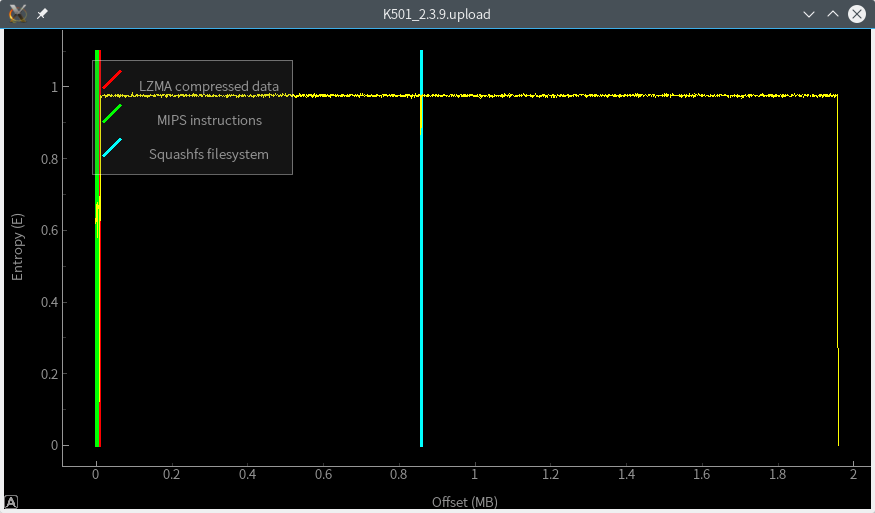
\includegraphics [width=100mm]{img/WeVO_K501_entropy.png}
\end{frame}

\begin{frame}
  \frametitle{0x02. 펌웨어 언팩}
  \framesubtitle{Let's walk on the binary}

  펌웨어 추출.
  binwalk 의 -e 옵션을 사용하여 펌웨어의 섹션들을 추출.
  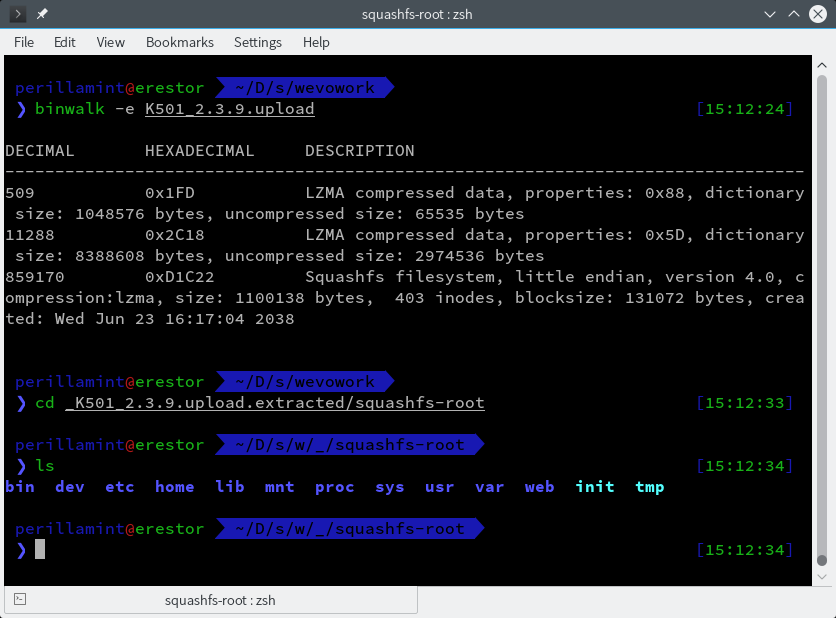
\includegraphics [width=100mm]{img/WeVO_K501_extracted.png}
\end{frame}

\section[Section]{바이너리 역공학}
\begin{frame}
  \frametitle{0x03. 대상 바이너리는 어디에}
  \framesubtitle{Init is always the first process}

  /etc/init.d/ 에는 init script 들이 존재한다.

  열어서 살펴보도록 하자.
  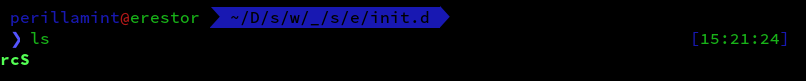
\includegraphics [width=100mm]{img/WeVO_K501_initscript.png}
\end{frame}

\begin{frame}
  \frametitle{0x03. 대상 바이너리는 어디에}
  \framesubtitle{Init is the first process}

  /etc/init.d/rcS 의 마지막 줄에서 webs 바이너리가 실행되는것을 볼 수 있다.

  해당 바이너리는 /bin/webs 에 위치한다.

  해당 바이너리를 분석해 보자.
\end{frame}

\begin{frame}
  \frametitle{0x04. 바이너리를 까보자}
  \framesubtitle{0x7F, 0x45, 0x4C, 0x46}

  readelf -h webs

  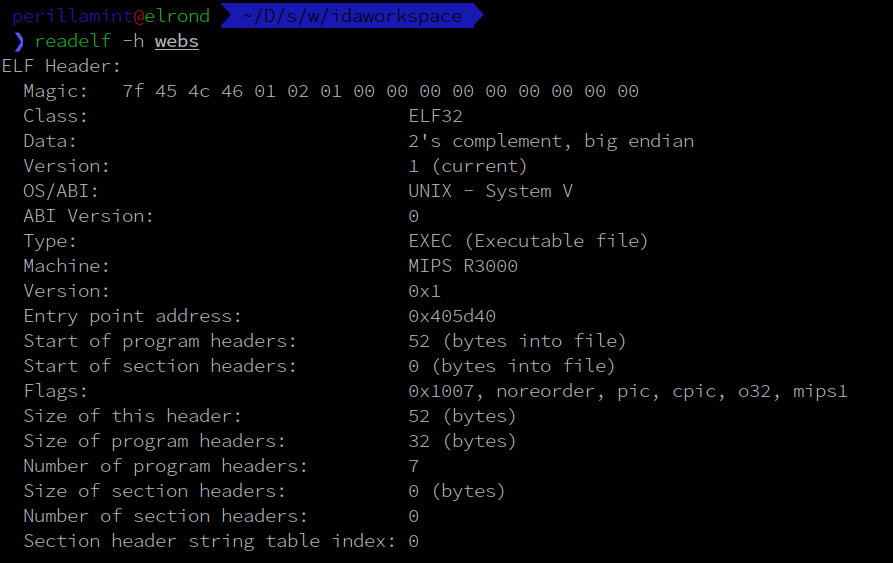
\includegraphics [width=100mm]{img/webs_readelf.png}

  MIPS32 Big endian ELF 바이너리이다.
\end{frame}

\begin{frame}
  \frametitle{0x05. 취약점을 찾아보자}
  \framesubtitle{Running everything as root is bad idea}

  IDA - Interactive DisAssembler
  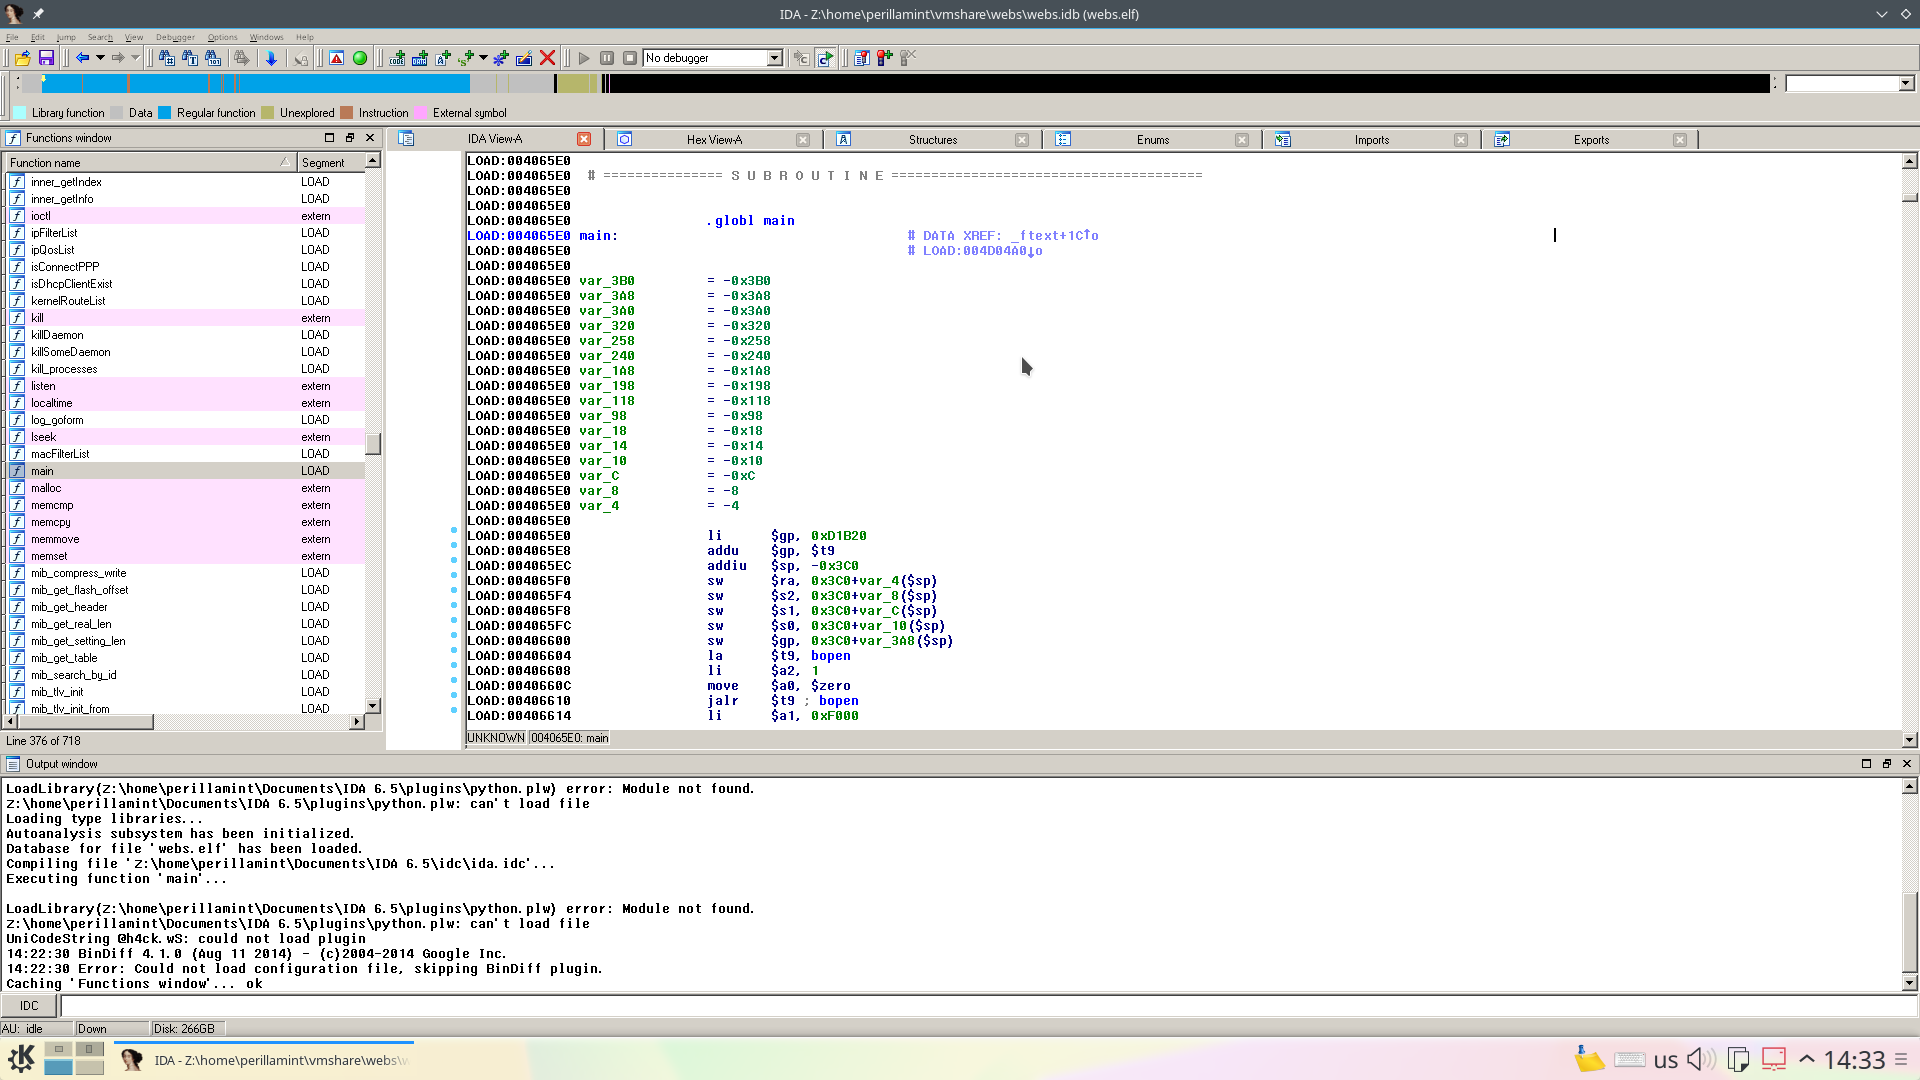
\includegraphics [width=100mm]{img/webs_idamain.png}
\end{frame}

\begin{frame}
  \frametitle{0x05. 취약점을 찾아보자}
  \framesubtitle{system(3) is TERRIBLE idea}

  공략 대상 라이브러리 콜: (취약할 것 같은 것들)
  \begin {itemize}
  \item system(3)
  \item sprintf(3)
  \item 기타 BoF 혹은 인젝션을 일으킬 수 있는 함수들
  \end{itemize}
\end{frame}

\begin{frame}
  \frametitle{0x05. 취약점을 찾아보자}
  \framesubtitle{system(3) is TERRIBLE idea}

  모든 길은 system(3) 으로?
  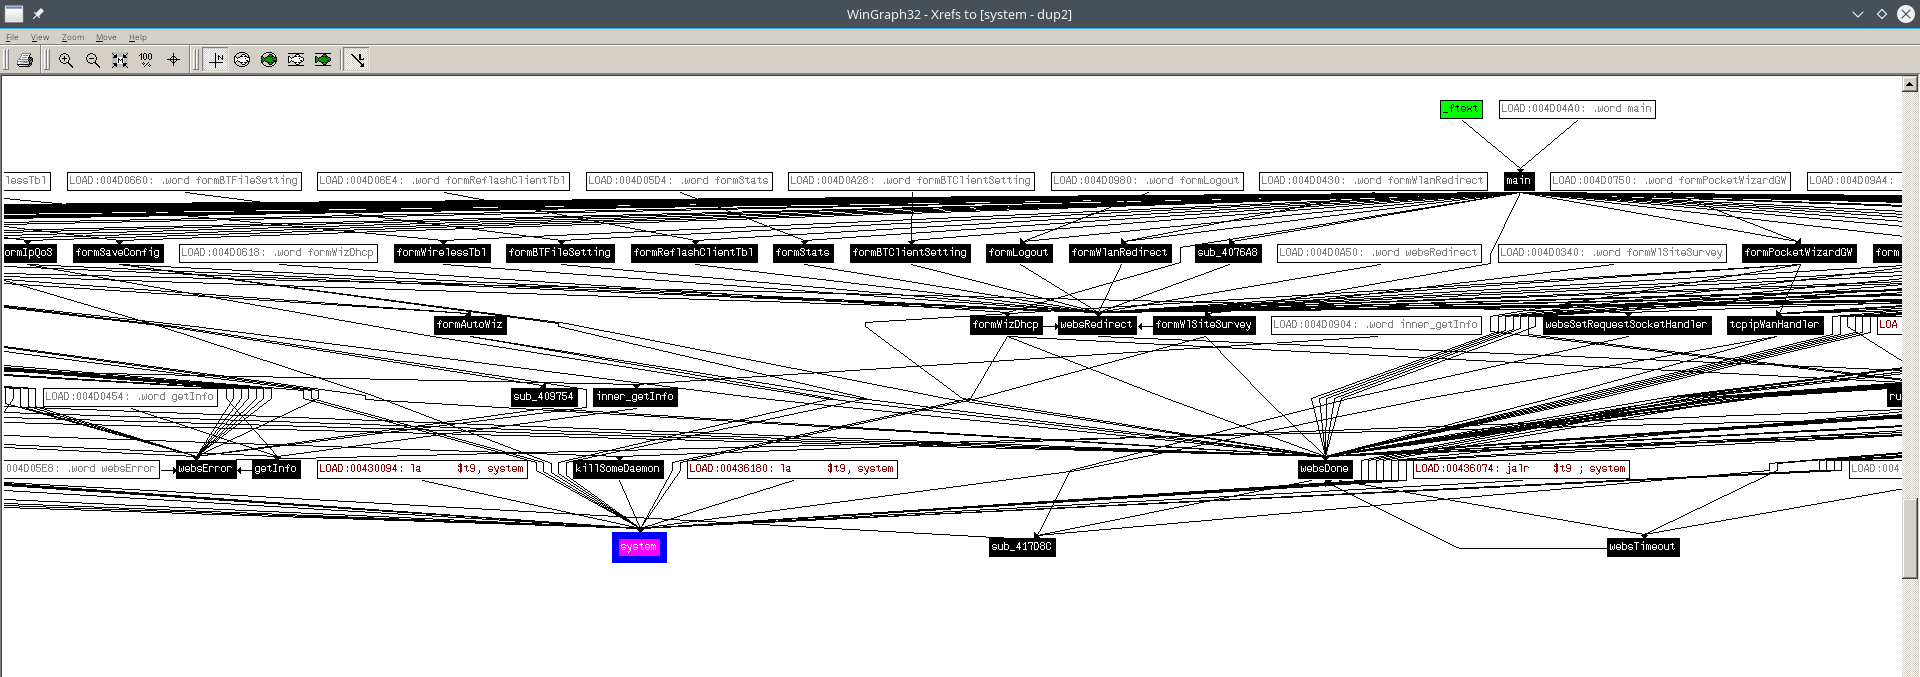
\includegraphics [width=100mm]{img/webs_system3_xref.png}
\end{frame}

\begin{frame}
  \frametitle{0x05. 취약점을 찾아보자}
  \framesubtitle{system(3) is TERRIBLE idea}

  DAFUQ? 사용자 입력에 sprintf(3) 과 system(3)?\linebreak
  해당 함수가 취약할 것 같다. 
  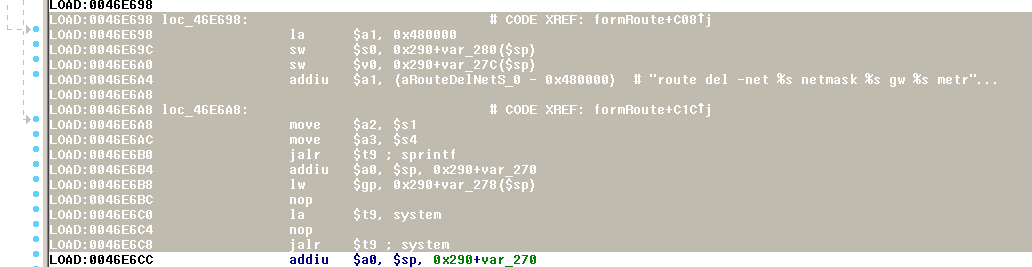
\includegraphics [width=100mm]{img/webs_system3_sprintf.png}
\end{frame}

\section[Section]{익스플로잇}
\begin{frame}
  \frametitle{0x06. 익스플로잇}
  \framesubtitle{Exploits of a Mom}

  입력을 넣어 보자.
  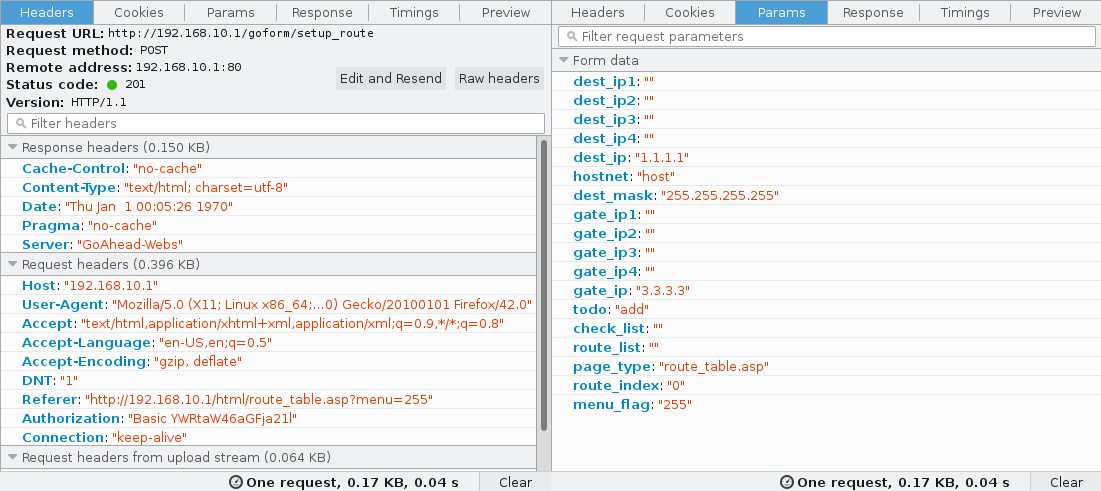
\includegraphics [width=100mm]{img/webs_setup_route.png}
\end{frame}

\begin{frame}
  \frametitle{0x06. 익스플로잇}
  \framesubtitle{Exploits of a Mom}

  POST dest\_ip 필드에 IP 어드레스 말고\linebreak
  ; wget -O /dev/null <someurl>;\# 을 넣어 보자.
  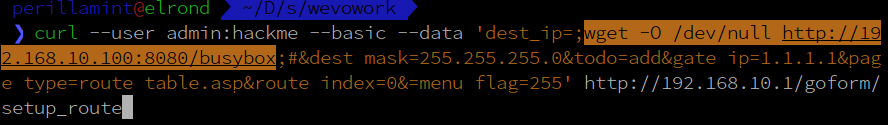
\includegraphics [width=100mm]{img/webs_shellinject_curl.png}
\end{frame}

\begin{frame}
  \frametitle{0x06. 익스플로잇}
  \framesubtitle{Exploits of a Mom}

  결과:\linebreak
  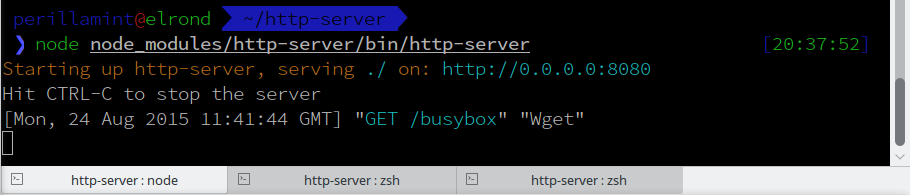
\includegraphics [width=100mm]{img/webs_shellinject.png}
\end{frame}

\begin{frame}
  \frametitle{0x07. 데모}
  \framesubtitle{Little bobby shells here}

\end{frame}

\section[Section]{왜 털렸는가}
\begin{frame}
  \frametitle{0x08. How system(3) and sprintf(3) hack works}
  \framesubtitle{Insane user inputs}

  How system(3) works:

  \begin{itemize}
  \item<1-> fork(2) 를 실행한다.
  \item<2->
    \only<2-2> {자식 프로세스는 /bin/sh 를 실행해, 인자를 셸 스크립트로 실행한다.}
    \only<3-> {자식 프로세스는 \textbf{/bin/sh} 를 실행해, 인자를 \textbf{셸 스크립트로} 실행한다.}
  \item<4-> 셸 스크립트 인젝션이 가능하다!
  \end{itemize}
\end{frame}

\begin{frame}
  \frametitle{0x08. How system(3) and sprintf(3) works}
  \framesubtitle{Insane user inputs}

  How sprintf(3) works:

  \begin{itemize}
  \item<1->주어진 템플릿에 주어진 데이터를 채워 넣은 것을\linebreak\textbf{크기 검사 없이} 주어진 버퍼에 집어넣는다
  \item<2->버퍼 오버플로우가 가능해진다.
  \end{itemize}
\end{frame}

\begin{frame}
  \frametitle{0x09. 막아보자}
  \framesubtitle{Defensive programming}

  \begin{itemize}
  \item<1->system(3) 대신 fork(2) \& execve(2) 를 사용해 자식 프로세스를 만든다.
  \item<2->snprintf(3) 을 사용해, 유저 데이터가 버퍼 밖으로 벗어나지 않도록 한다.
  \end{itemize}
\end{frame}

\section[Section]{보너스}

\begin{frame}
  \frametitle{0x09. 제조사가 펌웨어를 안 공개했다면?}
  \framesubtitle{Hardware sorcery}

  \begin{center}
    UART를 이용한 장치의 셸 접근

    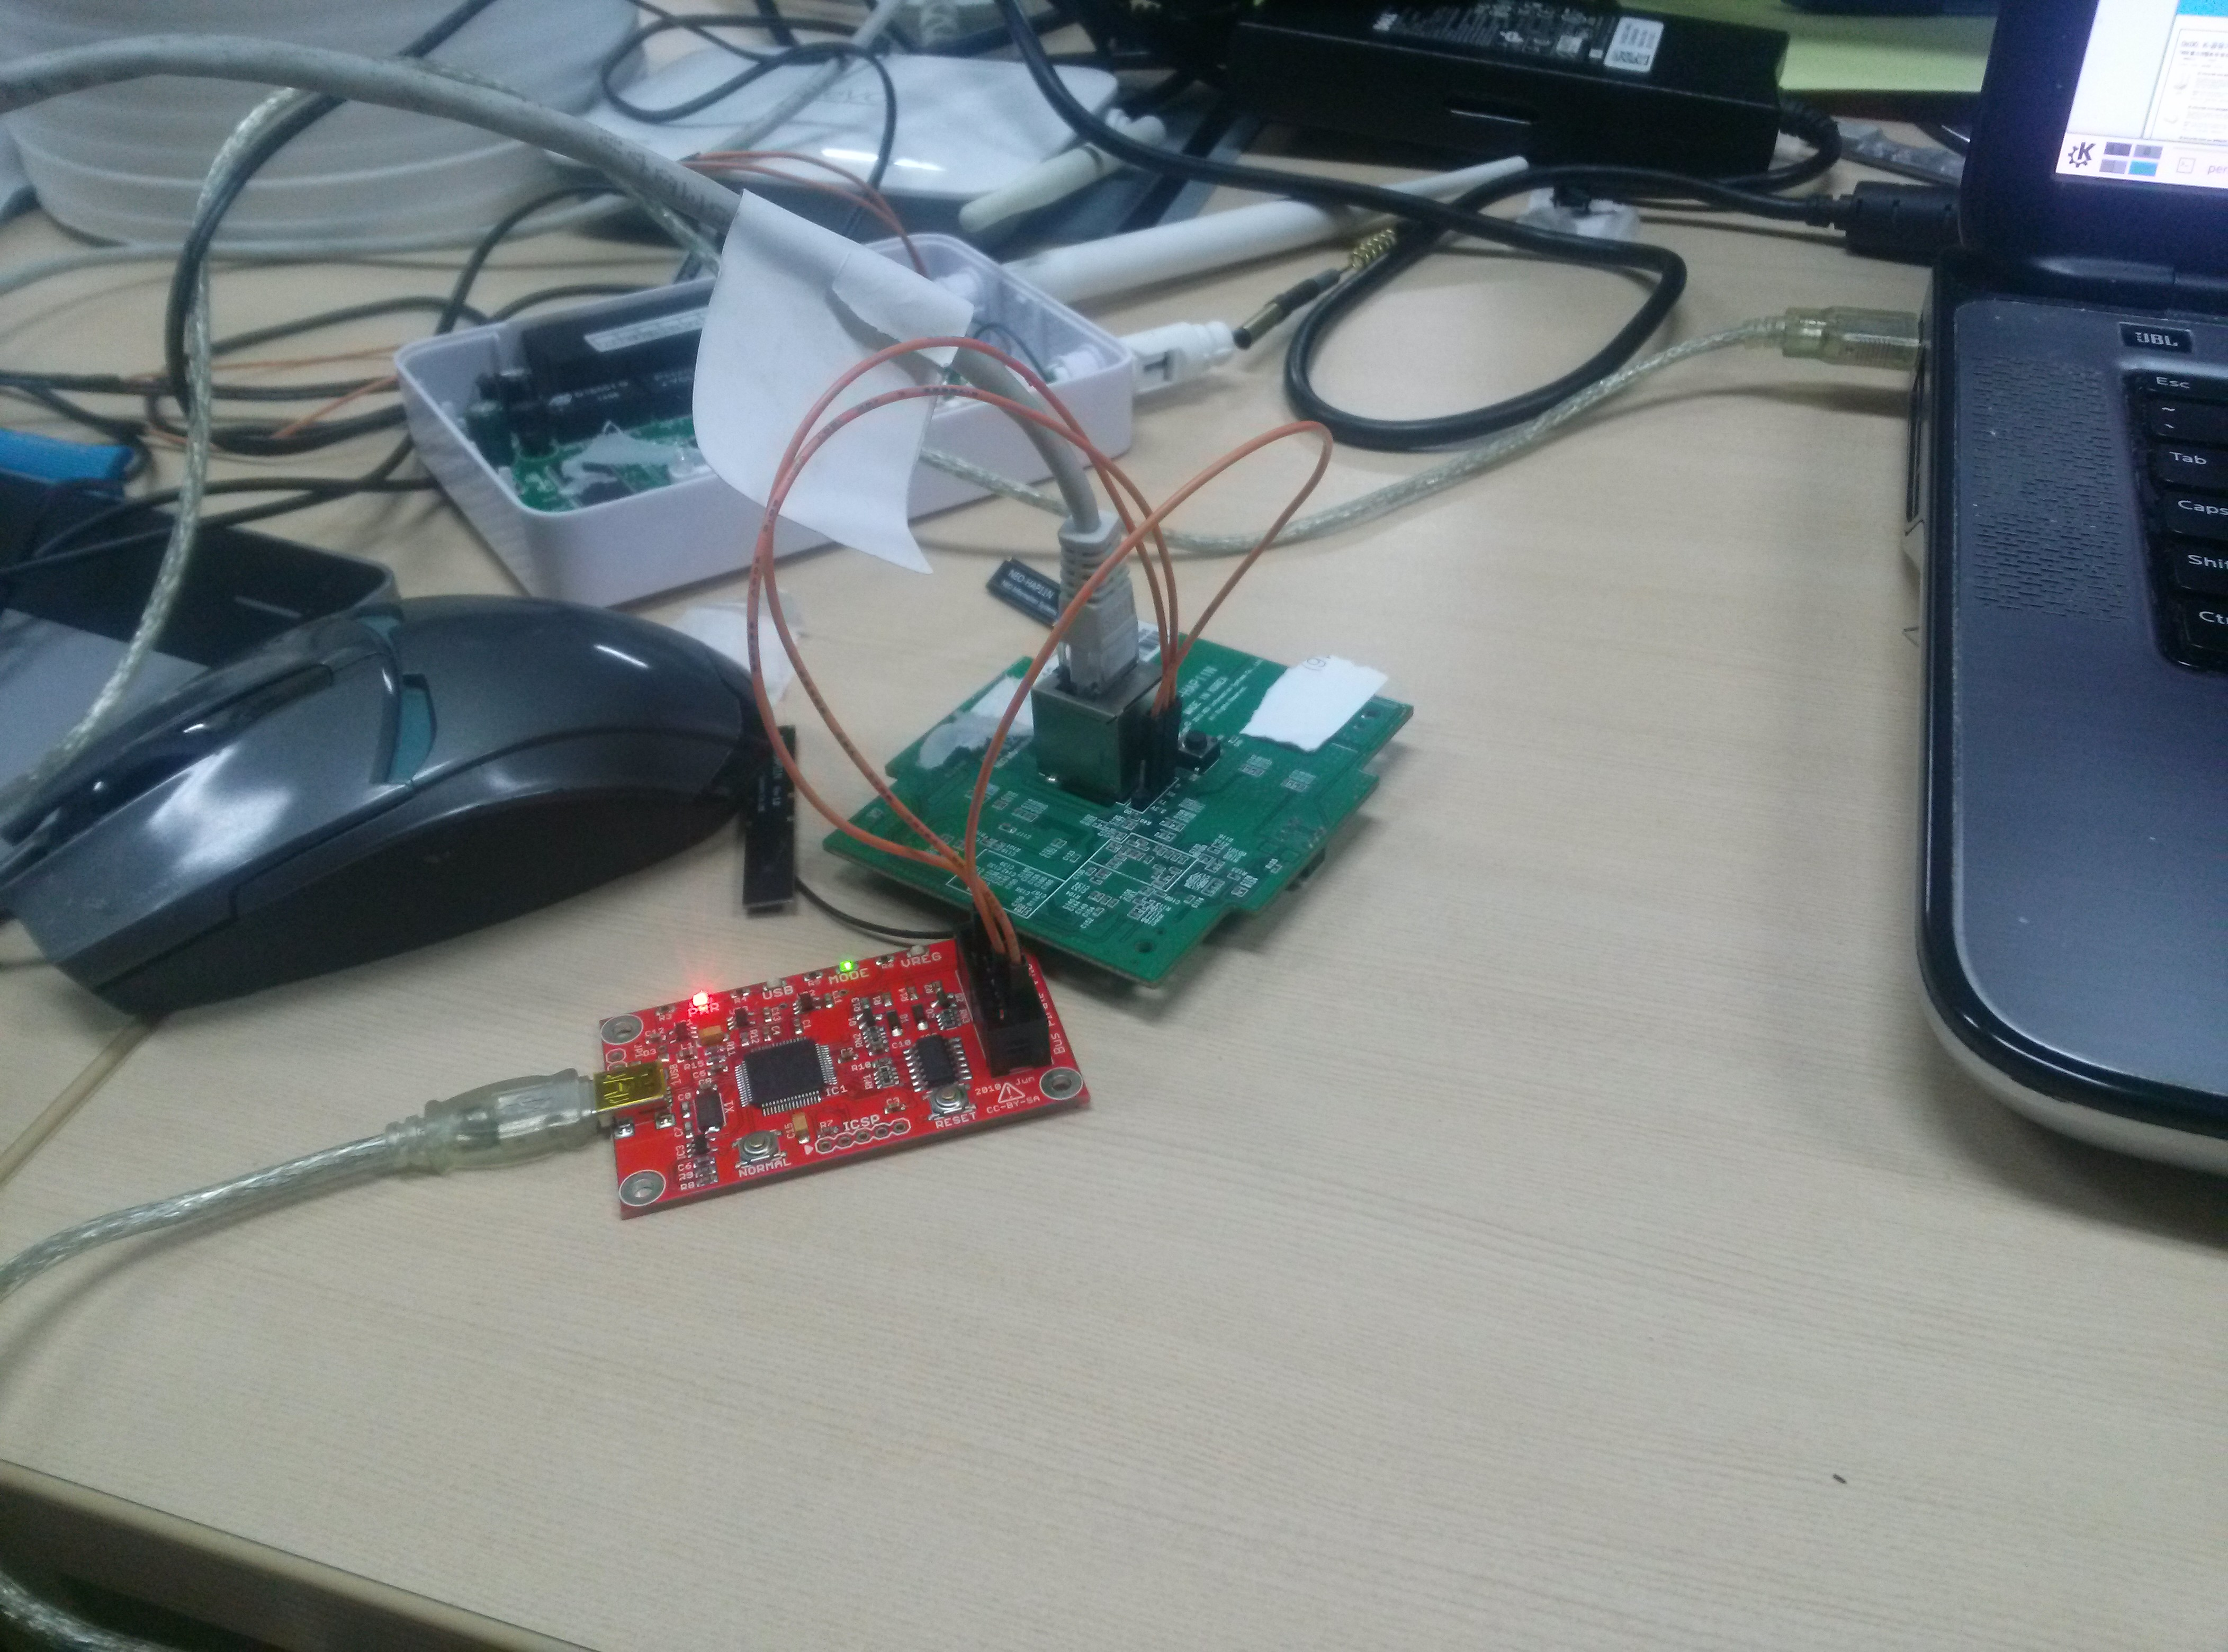
\includegraphics [width=70mm]{img/wrt-uart.jpeg}
  \end{center}
\end{frame}

\begin{frame}
  \frametitle{0x09. 제조사가 펌웨어를 안 공개했다면?}
  \framesubtitle{Hardware sorcery}

  \begin{center}
    I2C를 이용한 EEPROM 덤프

    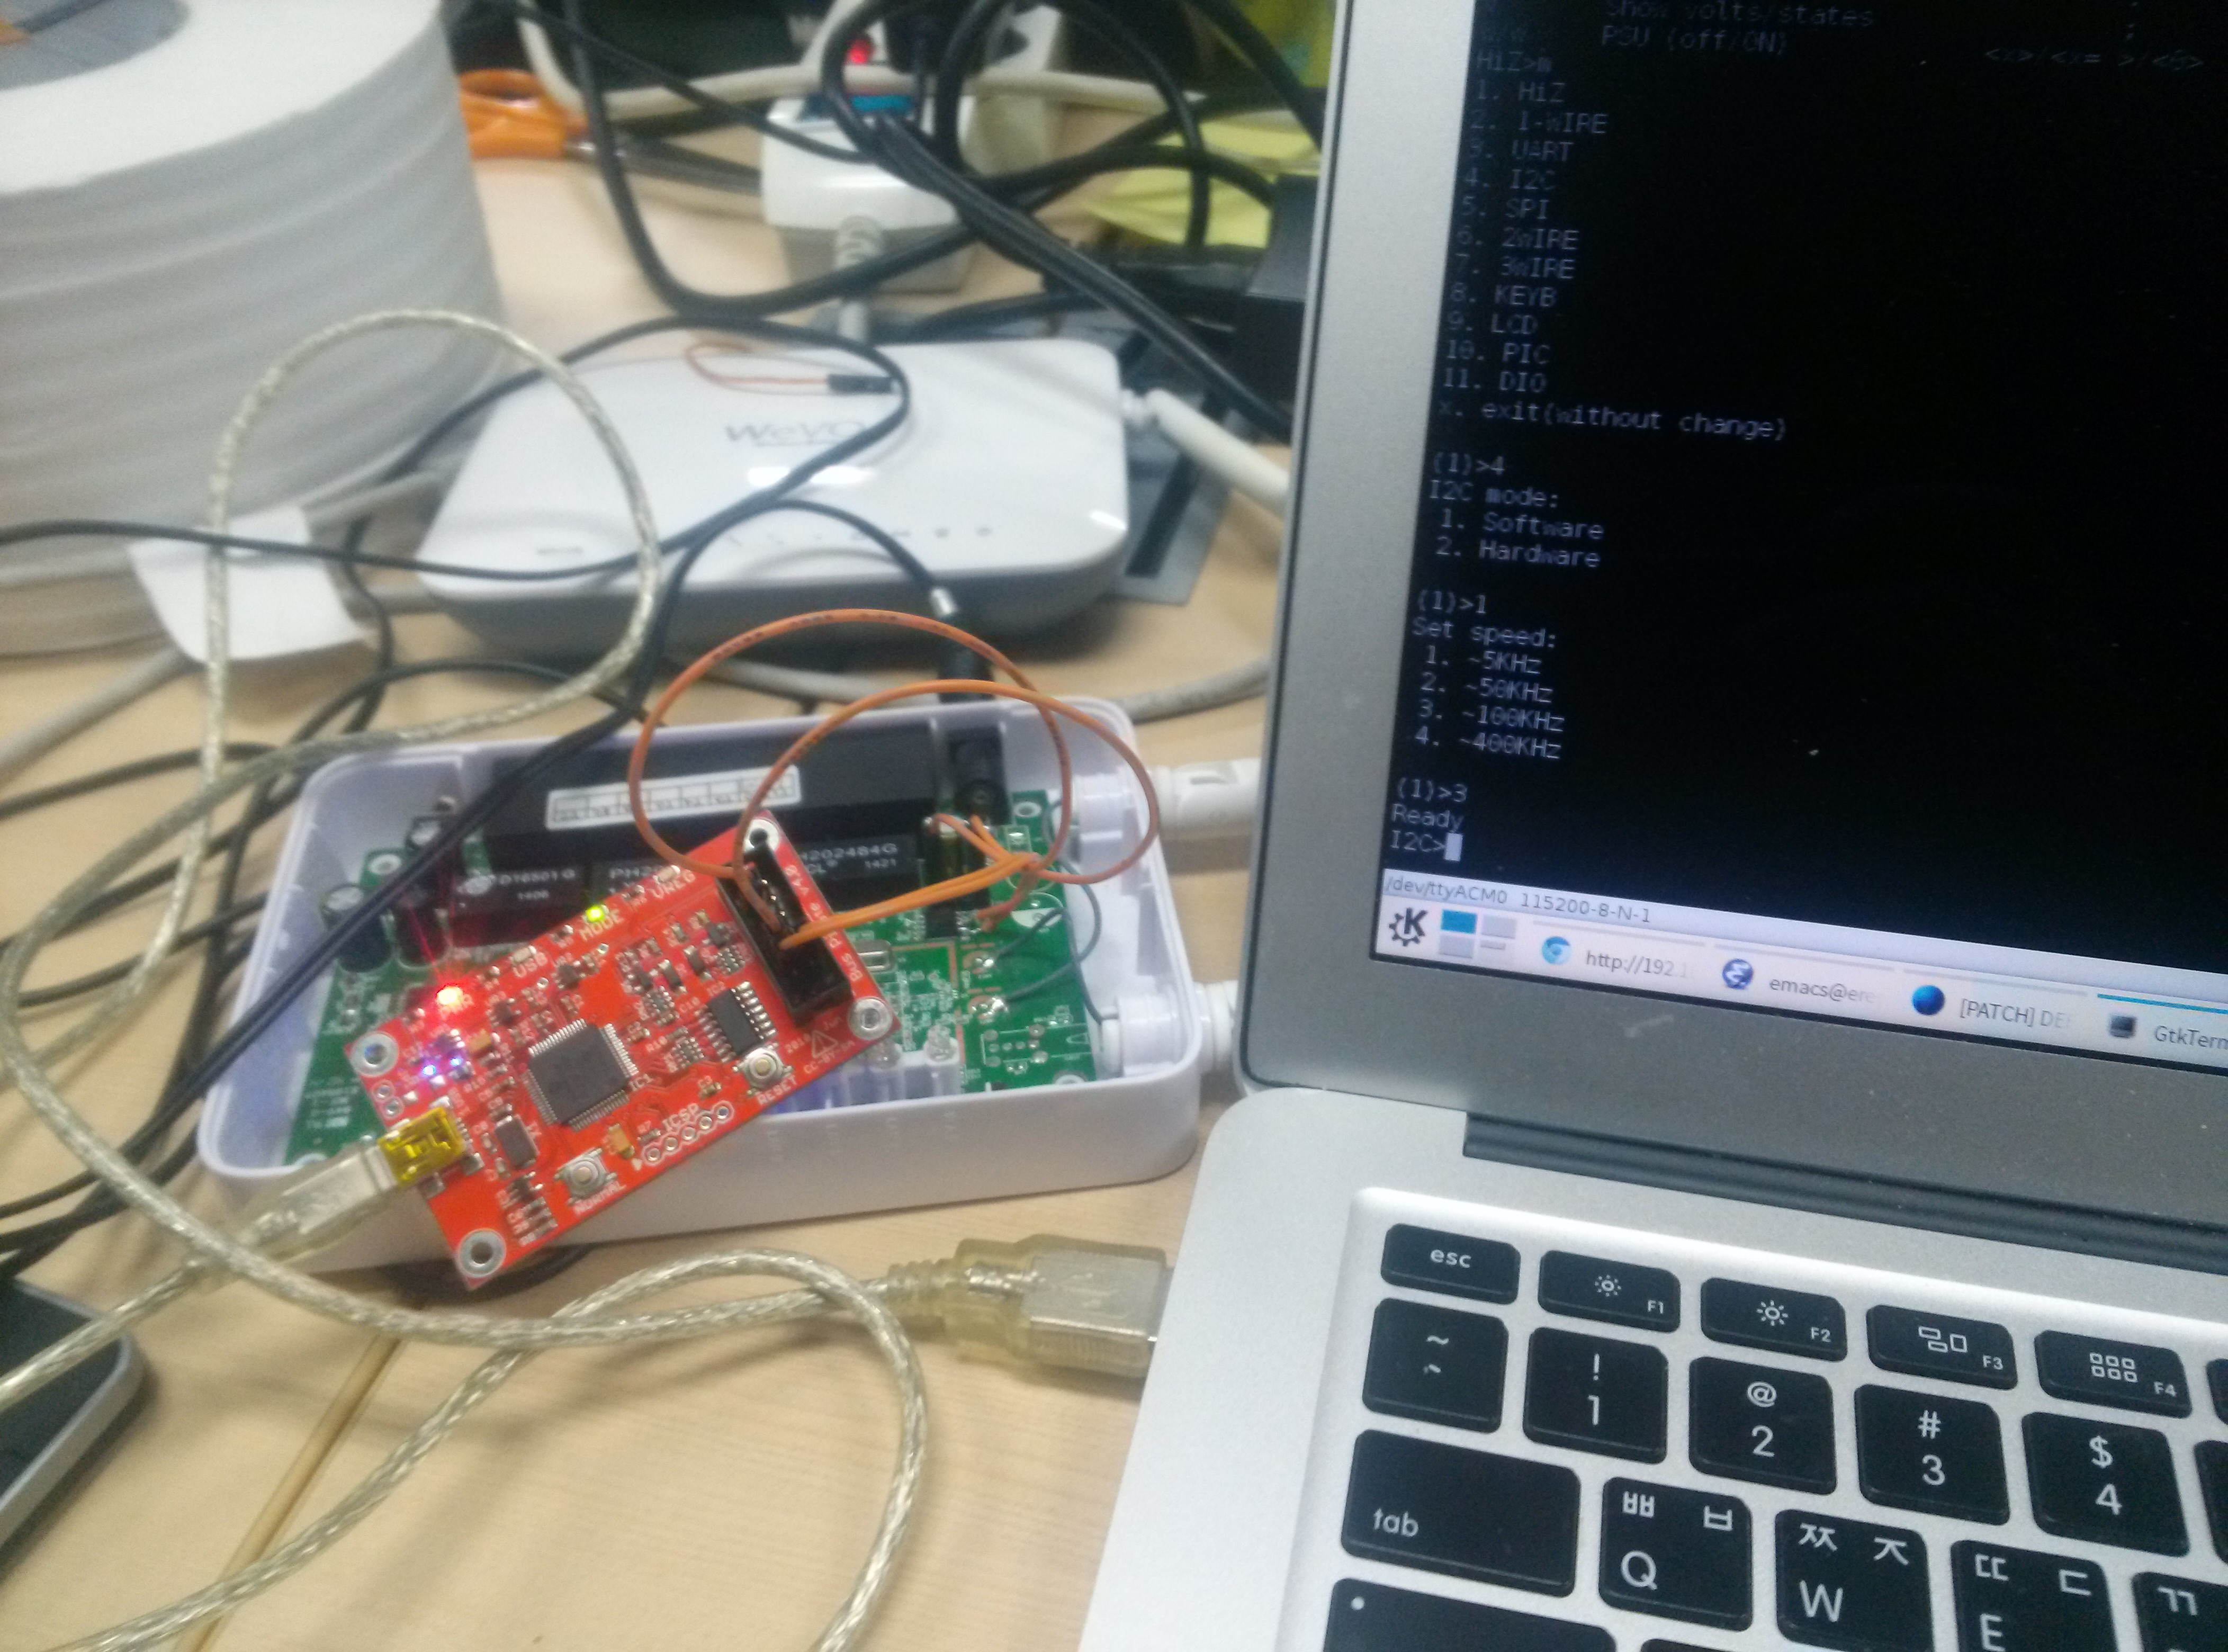
\includegraphics [width=70mm]{img/wrt-i2c.jpeg}
  \end{center}
\end{frame}

\begin{frame}
  \frametitle{0x0A. Hardcoded \& Default passwords}
  \framesubtitle{One password to rule them all}

  \begin{center}
    어처구니없는 모 빌트인 홈 라우터의 하드코드된 백도어 패스워드

    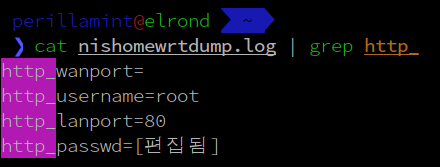
\includegraphics [width=100mm]{img/homeap_nvram.png}
  \end{center}
\end{frame}

\begin{frame}
  \frametitle{0x0A. Hardcoded \& Default passwords}
  \framesubtitle{One password to rule them all}

  \begin{center}
    그리고... 기본 루트 암호로 열려있는 텔넷....

    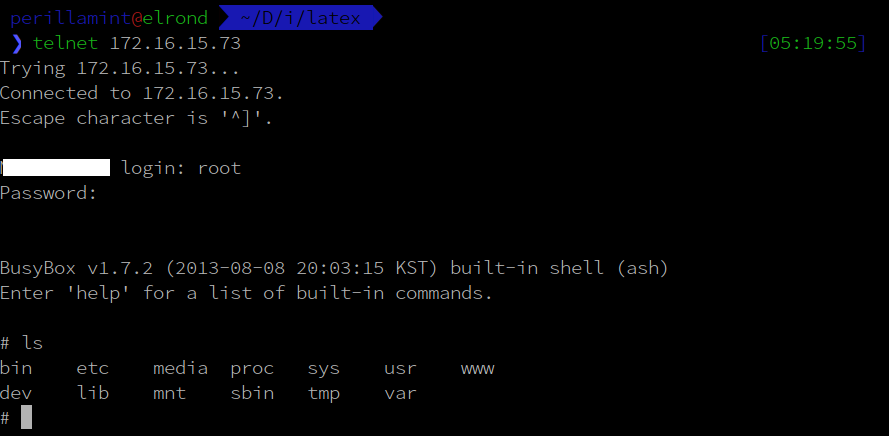
\includegraphics [width=100mm]{img/homeap_telnet.png}
  \end{center}
\end{frame}

\begin{frame}
  \frametitle{0x0A. Hardcoded \& Default passwords}
  \framesubtitle{One password to rule them all}

  \begin{center}
    KT 하이브리드 에그의 개발용 인터페이스
    \linebreak
    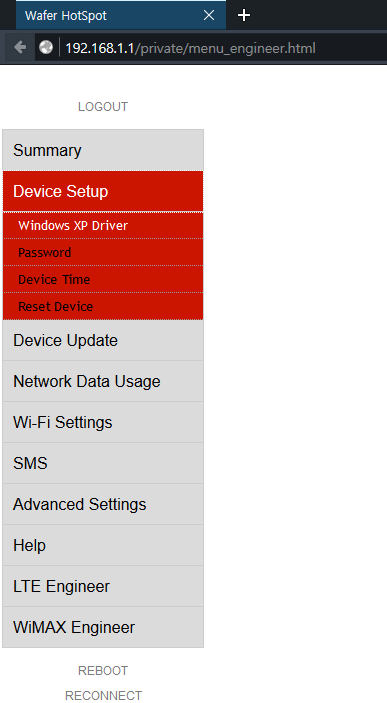
\includegraphics [height=50mm]{img/hybridegg.png}
  \end{center}
\end{frame}

\section[Section]{결론}
\begin{frame}
  \frametitle{0x0B. 결론}
  \framesubtitle{}

  \begin{itemize}
  \item<1->프로그래밍을 할 때, Malicious input 에 대비해야한다.
  \item<2->만약, 인젝션 공격을 허용하지 않을 수 있는 방법이 있다면, 그 방법을 택한다.
  \item<3->하드코드된 관리용 백도어는, 관리자 뿐만 아니라, 공격자도 이용할 수 있음을 생각해야한다.
  \end{itemize}
\end{frame}

\begin{frame}
  \frametitle{0x0C. 소비자 레벨에서의 대안은?}
  \framesubtitle{Stock firmware sucks}

  \begin{center}
    
\includegraphics [width=50mm]{img/openwrt-logo.png}
    \linebreak
    \linebreak
    
\includegraphics [width=50mm]{img/librewrt.png}
    \linebreak
    \linebreak
    
\includegraphics [width=50mm]{img/dd-wrt-logo.png}
  \end{center}
\end{frame}

\begin{frame}
  \frametitle{0x0D. 끝}
  \framesubtitle{FIN}

  \begin{center}
    Q \& A
  \end{center}
\end{frame}

\begin{frame}
  \frametitle{0x0E. License}
  \framesubtitle{}
  Copyright (C)  2015 perillamint\linebreak
  Permission is granted to copy, distribute and/or modify this document
  under the terms of the GNU Free Documentation License, Version 1.3
  or any later version published by the Free Software Foundation;\linebreak
  with no Invariant Sections, no Front-Cover Texts, and no Back-Cover Texts.
  A copy of the license is included in the section entitled "GNU
  Free Documentation License".
  \linebreak
  \linebreak
  Repository address:\linebreak
  \url{https://github.com/perillamint/K-HomeWRT-hack}
  \linebreak
  \linebreak
  
\includegraphics [width=30mm]{img/gfdl-logo-small.png}
\end{frame}

\end {document}
